\section{Prompts in \sys}
\label{appendix:prompts_in_autoprep}

In this Section, we present the prompts used by \sys and our compared baselines. We omit the operator definition in the prompt due to the space limit, a complete definition can be found in our published code repository\footnote{\url{https://anonymous.4open.science/r/DeepPrep-0432/src/physicalop/data_transform.py}}. For each method, we provide two demonstrations as supervision for In-Context Learning, which is also omitted.

\subsection{Prompt Construction and State Representation of \sys}
\label{subsec:appendix_deepprep_prompt}

We present the detailed prompts of \sys.

%!TEX root = ../../main.tex
\begin{figure}[!t]
    \centering 
    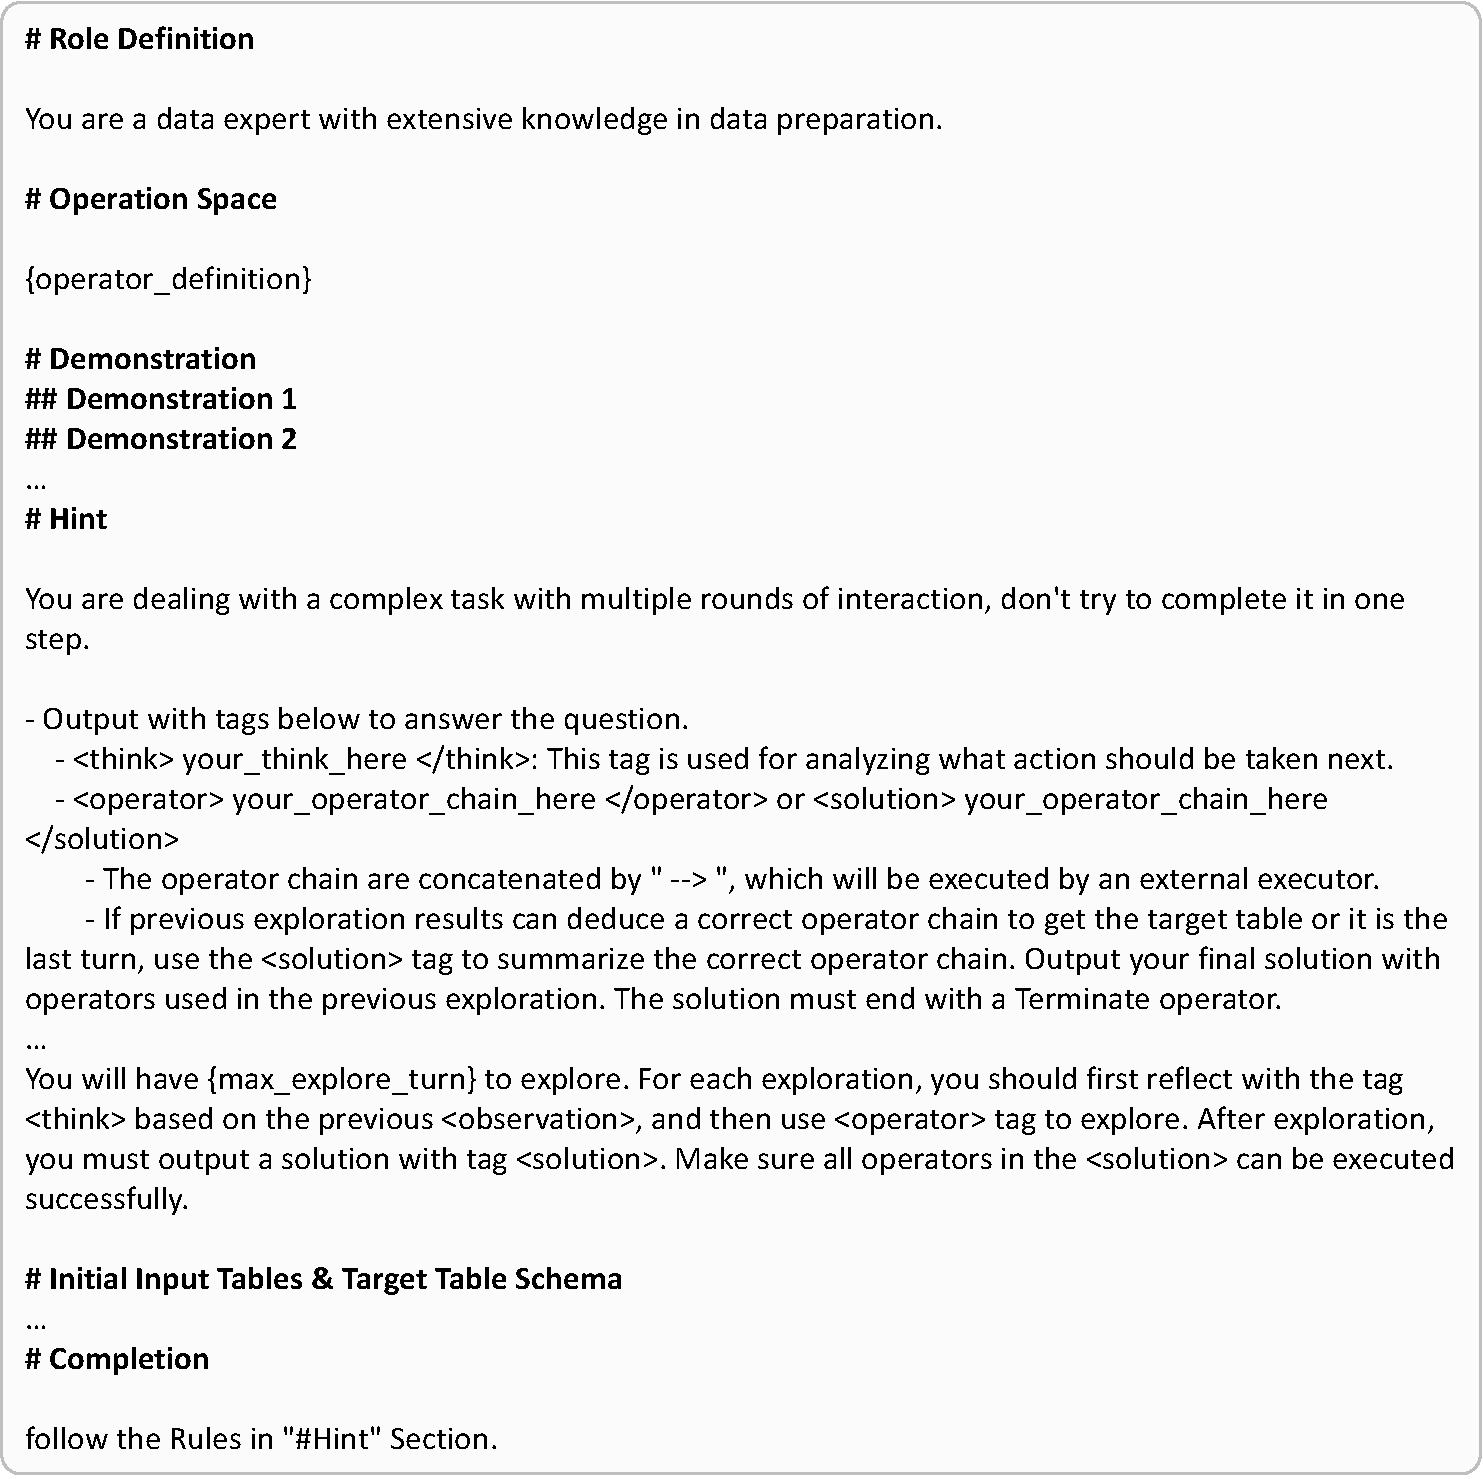
\includegraphics[width=1.01\columnwidth]{appendix/figures/fig/deepprep_initial_prompt.pdf}
    \vspace{-2em}
    \caption{Prompt of \sys.
    }
    \label{fig:deepprep_initial_prompt}
    \vspace{-1em}
\end{figure}

%!TEX root = ../../main.tex
\begin{figure*}[!t]
    \centering 
    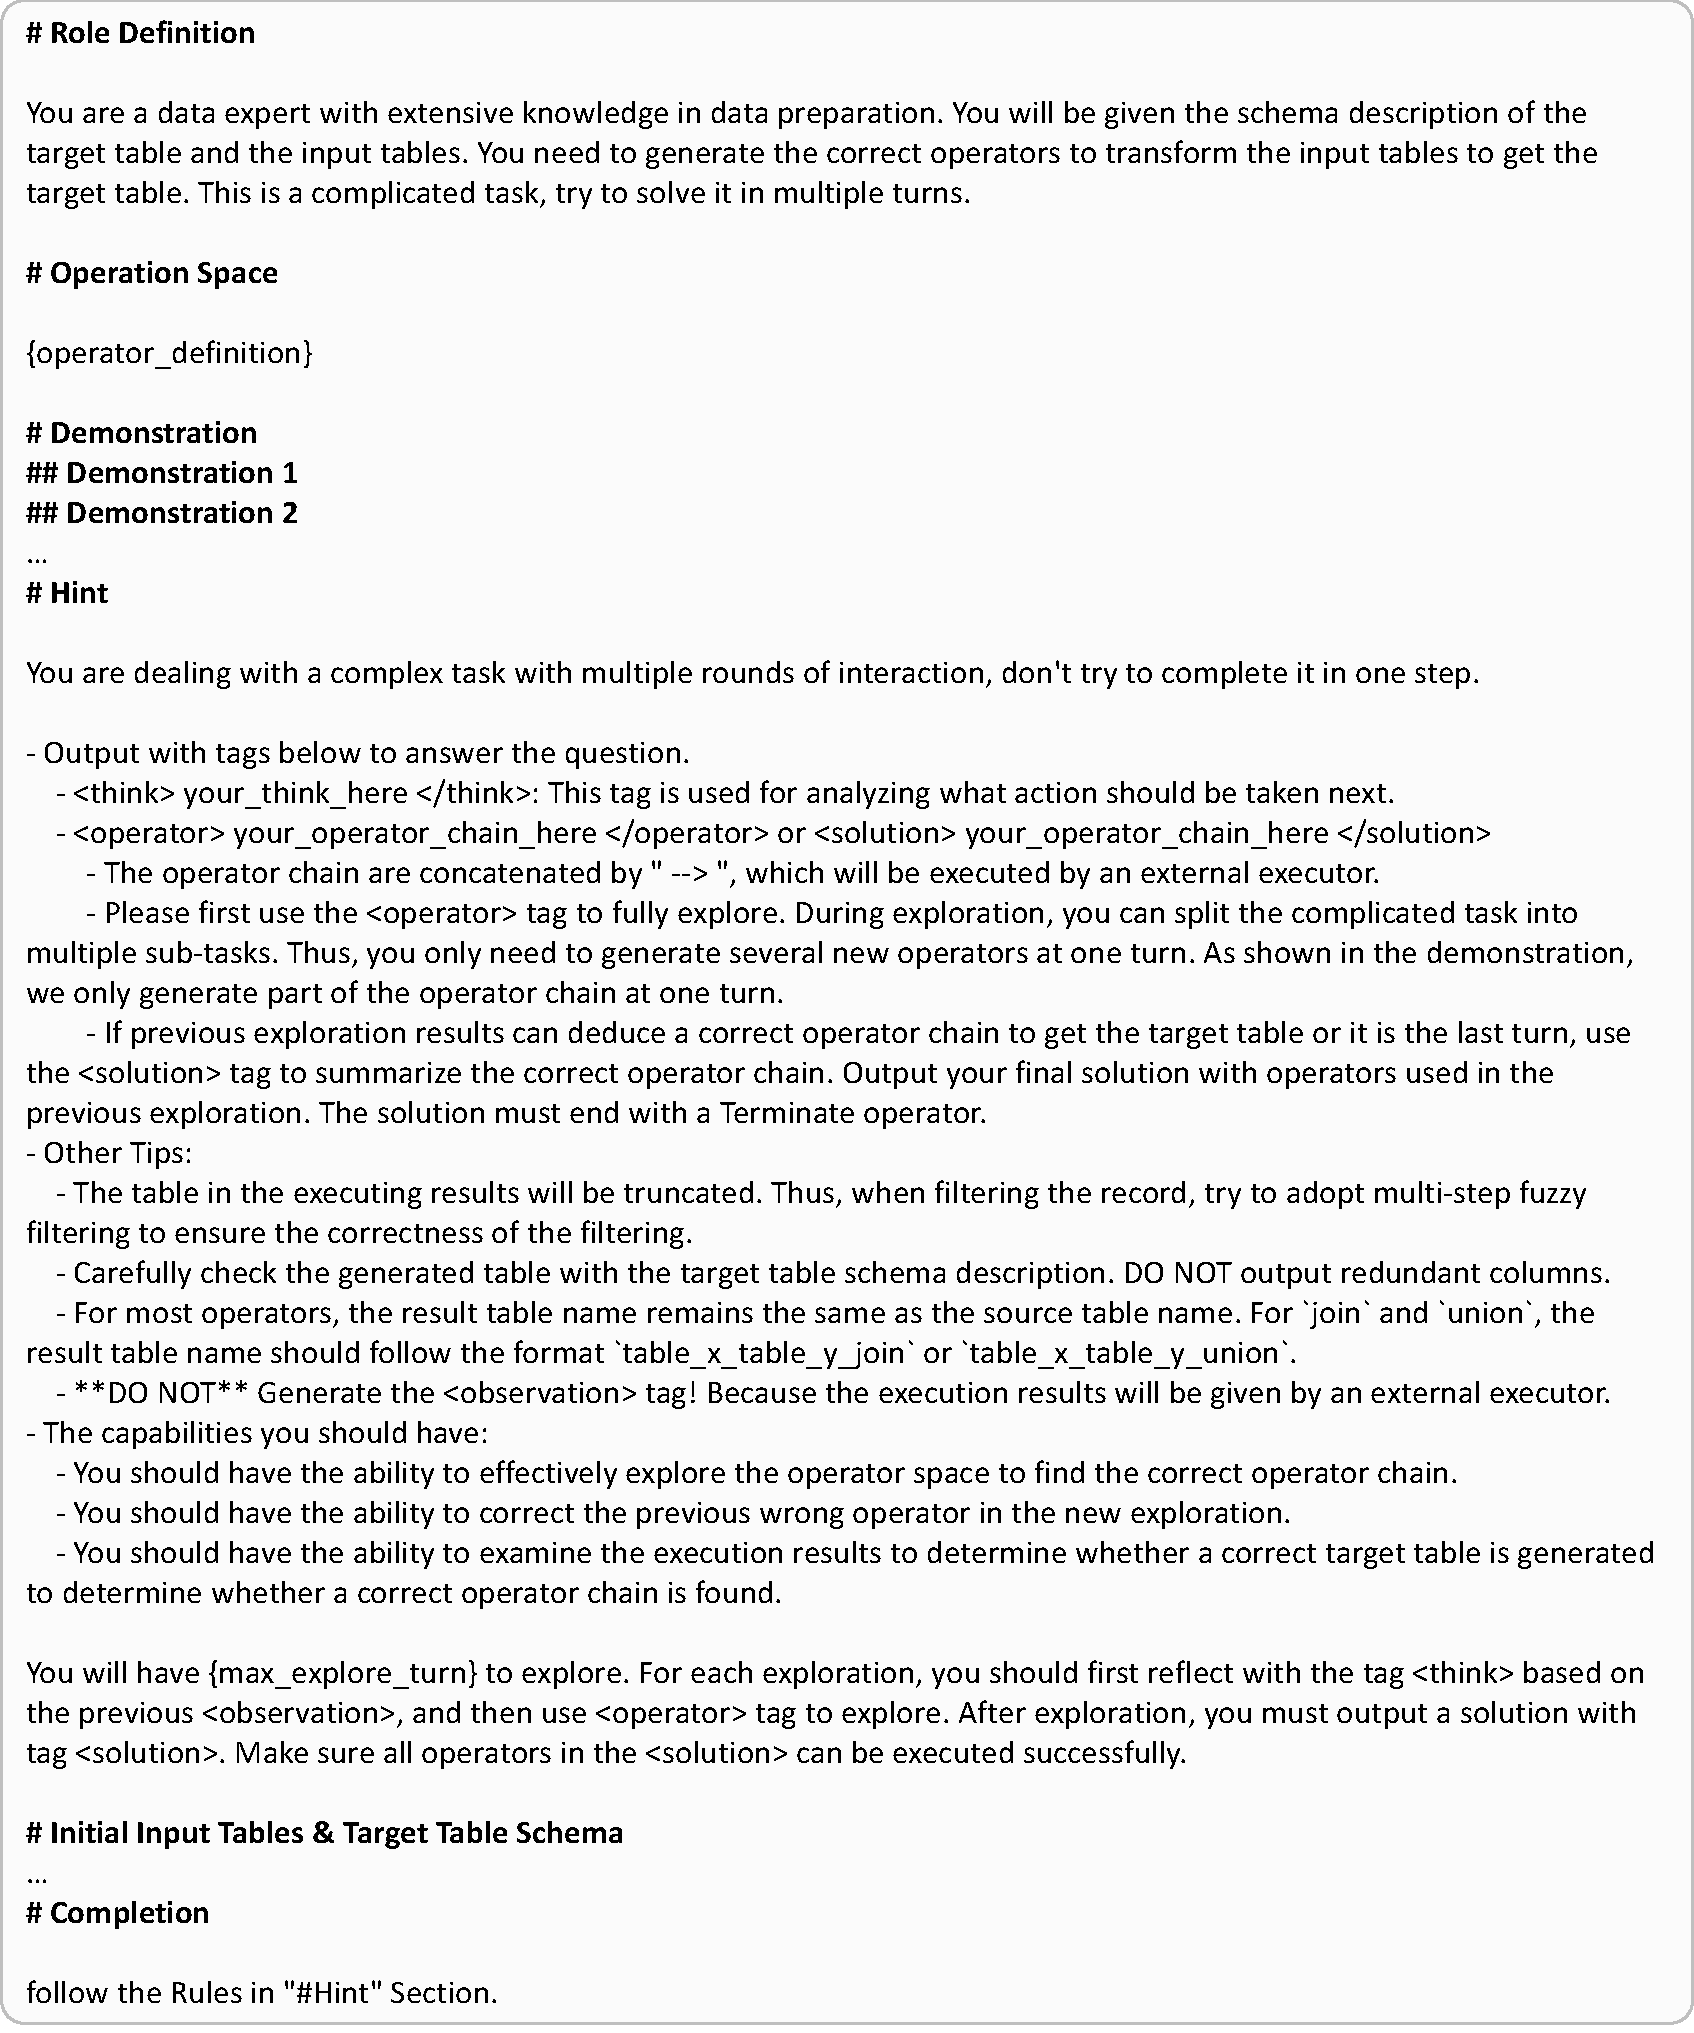
\includegraphics[width=0.85\textwidth]{appendix/figures/fig/deepprep_trajectory_prompt.pdf.pdf}
    \vspace{-0.5em}
    \caption{The trajectory prompt template of \sys during multi-turn interaction. After each exploration turn, the execution results of the operator chain are appended as \texttt{<observation>} blocks, which contain the sampled intermediate table data and a \texttt{<reminder>} tag indicating the remaining exploration turns. The agent can then analyze the observation with \texttt{<think/>} and either continue exploring with \texttt{<operator>} or output the final pipeline with \texttt{<solution>}.
    }
    \label{fig:deepprep_trajectory_prompt}
    % \vspace{-1em}
\end{figure*}


\stitle{Initial Prompt Construction.}
As shown in Figure~\ref{fig:deepprep_initial_prompt}, the initial prompt of \sys consists of a system prompt and a user prompt.

The system prompt contains four components:
(1) {Role Definition}. The model is assigned the role of a ``data expert with extensive knowledge in data preparation,'' establishing the task context for autonomous data preparation.
(2) {Operation Space}. The full set of operator definitions $\mathcal{O}$ is provided, including each operator's name, parameters, and functional description. This enables the model to generate syntactically correct operator instances.
(3) {Demonstration}. Two few-shot examples are included to illustrate the interaction protocol. Each demonstration shows how to use the \texttt{<think>} tag for analysis, the \texttt{<operator>} tag for exploration, and the \texttt{<solution>} tag for finalizing the pipeline.
(4) {Hint}. This section specifies the interaction protocol, including: (a) the usage of \texttt{<think/>} for analyzing the current state and planning the next step, (b) the distinction between \texttt{<operator>} for exploration and \texttt{<solution>} for the final pipeline, (c) the constraint that each turn's operator chain must be generated from scratch rather than cached from previous turns, (d) naming conventions for intermediate tables produced by \texttt{Join} and \texttt{Union} operations and (e) the maximum number of exploration turns (\texttt{max\_explore\_turn}).

The user prompt contains two components:
(1) \textbf{Initial Input Tables}: The source tables are serialized into a Markdown-formatted representation. Each table is labeled with a name (\eg \texttt{table\_1}) and includes the column headers and sampled row data. For source tables, we sample up to 20 columns and 20 rows to control token usage while preserving sufficient information for the model to understand the table structure and content.
(2) \textbf{Target Table Schema Description}: Instead of providing the full target table content, we provide a structured schema description that includes: (a) a natural language task description explaining the transformation intent; and (b) for each target column, its name, a semantic description, and a list of requirements (\eg ``Distinct values for each row,'' ``Non-negative integer values''). This schema-only representation avoids leaking the target table values while providing sufficient guidance for the model to construct the correct pipeline.

\stitle{State Representation during Interaction.}
As shown in Figure~\ref{fig:deepprep_trajectory_prompt}, during the multi-turn interaction process, the prompt is incrementally updated with execution feedback.
Specifically, after each exploration turn where the agent generates an operator chain wrapped in \texttt{<operator>} tags, the environment executes the operators and returns an \texttt{<observation>} block containing:
(1) \textbf{Intermediate Table Data}: The execution results of each operator in the chain are serialized. For each operator, both the operator string and the resulting table sample are shown. For intermediate tables, we sample up to 8 columns and 5 rows to further control token usage, as intermediate tables tend to be more numerous and their detailed content is less critical for high-level planning.
(2) \textbf{Reminder}: A \texttt{<reminder>} tag is appended to the observation, indicating the remaining exploration turns and prompting the agent to either continue exploring with \texttt{<operator>} or finalize the pipeline with \texttt{<solution>}.

\stitle{Schema Handling.}
A key design decision in our prompt construction is that \textbf{intermediate table schemas are not explicitly included} in the prompt. Instead, the schema information is implicitly conveyed through the sampled data of intermediate tables. For example, when a \texttt{GroupBy} operator produces an intermediate table, the column names and data types are evident from the sampled rows shown in the \texttt{<observation>} block. This design choice is motivated by two considerations:
(1) Including explicit schema descriptions for every intermediate table would significantly increase the prompt length, especially for tasks with long pipelines that produce many intermediate states.
(2) The sampled data provides sufficient schema information for the model to reason about subsequent operations, as column names are directly visible in the table header and data types can be inferred from the sample values.

\stitle{Table Content Sampling Strategy.}
To handle large tables within the context window constraints of LLMs, we employ a differentiated sampling strategy:
(1) For \textbf{source tables} (in the initial prompt), we sample up to 20 columns and 20 rows. This provides the model with a comprehensive view of the input data structure and content.
(2) For \textbf{intermediate tables} (in the \texttt{<observation>} blocks), we sample up to 8 columns and 5 rows. Since intermediate tables are produced at each exploration turn and multiple operators may be executed per turn, a more aggressive sampling strategy is necessary to prevent context overflow. The reduced sample size still preserves the essential schema and value distribution information needed for the model to evaluate the correctness of its operations.
(3) When the number of columns exceeds the sampling limit, we truncate the remaining columns and append ``\texttt{...}'' to indicate the truncation. Similarly, when the number of rows exceeds the limit, we append ``\texttt{......}'' after the last sampled row.

\stitle{Failed Branch Reuse.}
\revise{During tree-based exploration, failed branches are preserved with their error traces and reused to inform future exploration. Specifically, when a branch produces an execution error, the \texttt{<observation>} block containing the error message is retained in the trajectory, allowing the agent to avoid repeating the same failed operator chain in subsequent branches (see Example~\ref{exam:agentic_reasoning_example}).}

\subsection{Prompts of Baselines}
\label{subsec:prompts_of_baselines}

\begin{figure}[!t]
    \centering 
    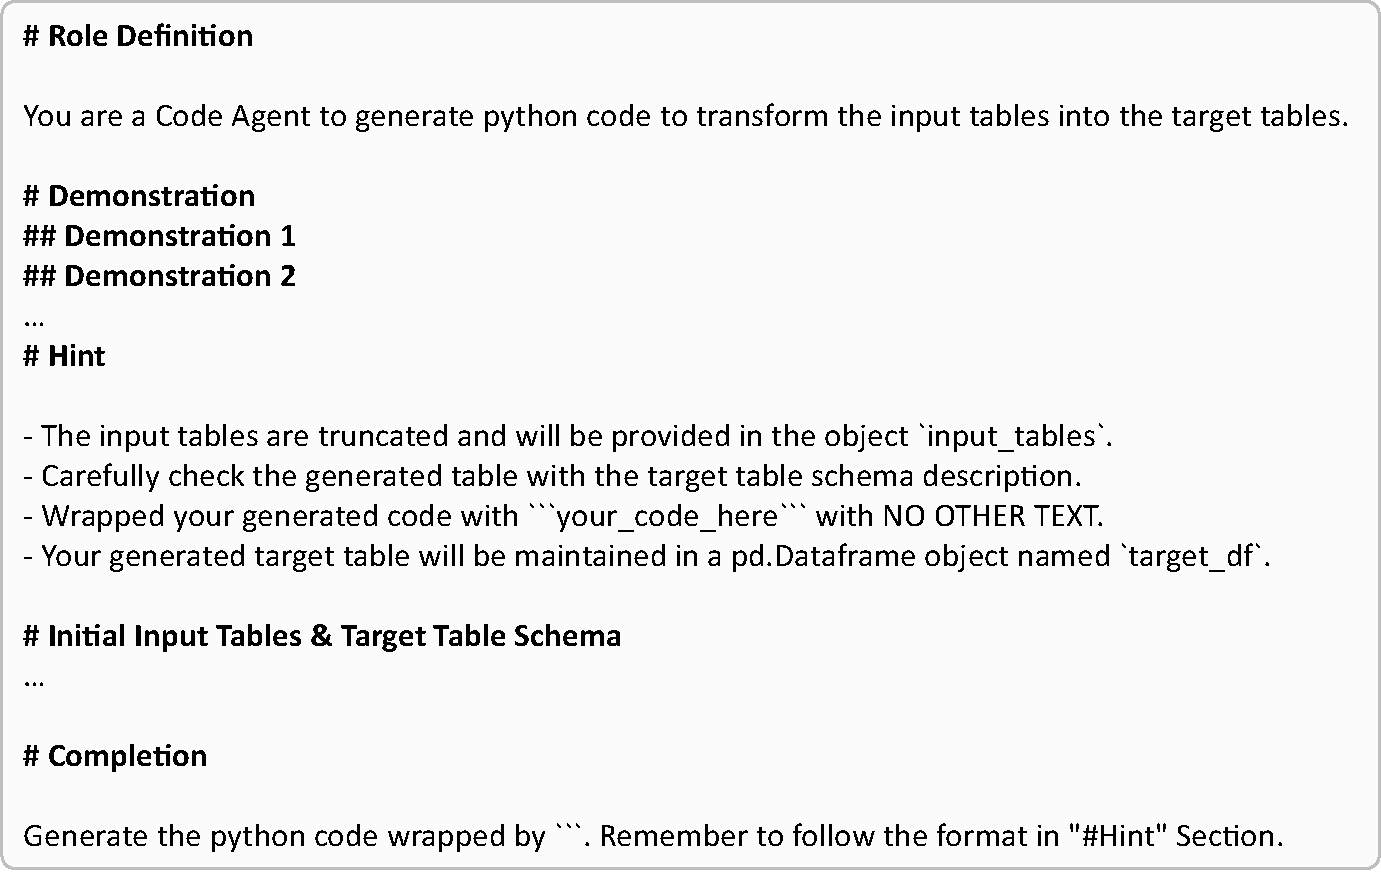
\includegraphics[width=0.99\columnwidth]{appendix/figures/fig/code_gen_prompt.pdf}
    \vspace{-1em}
    \caption{Prompt of CodeGen.
    }
    \label{fig:code_gen_prompt}
    % \vspace{-1em}
\end{figure}

\begin{figure}[!t]
    \centering 
    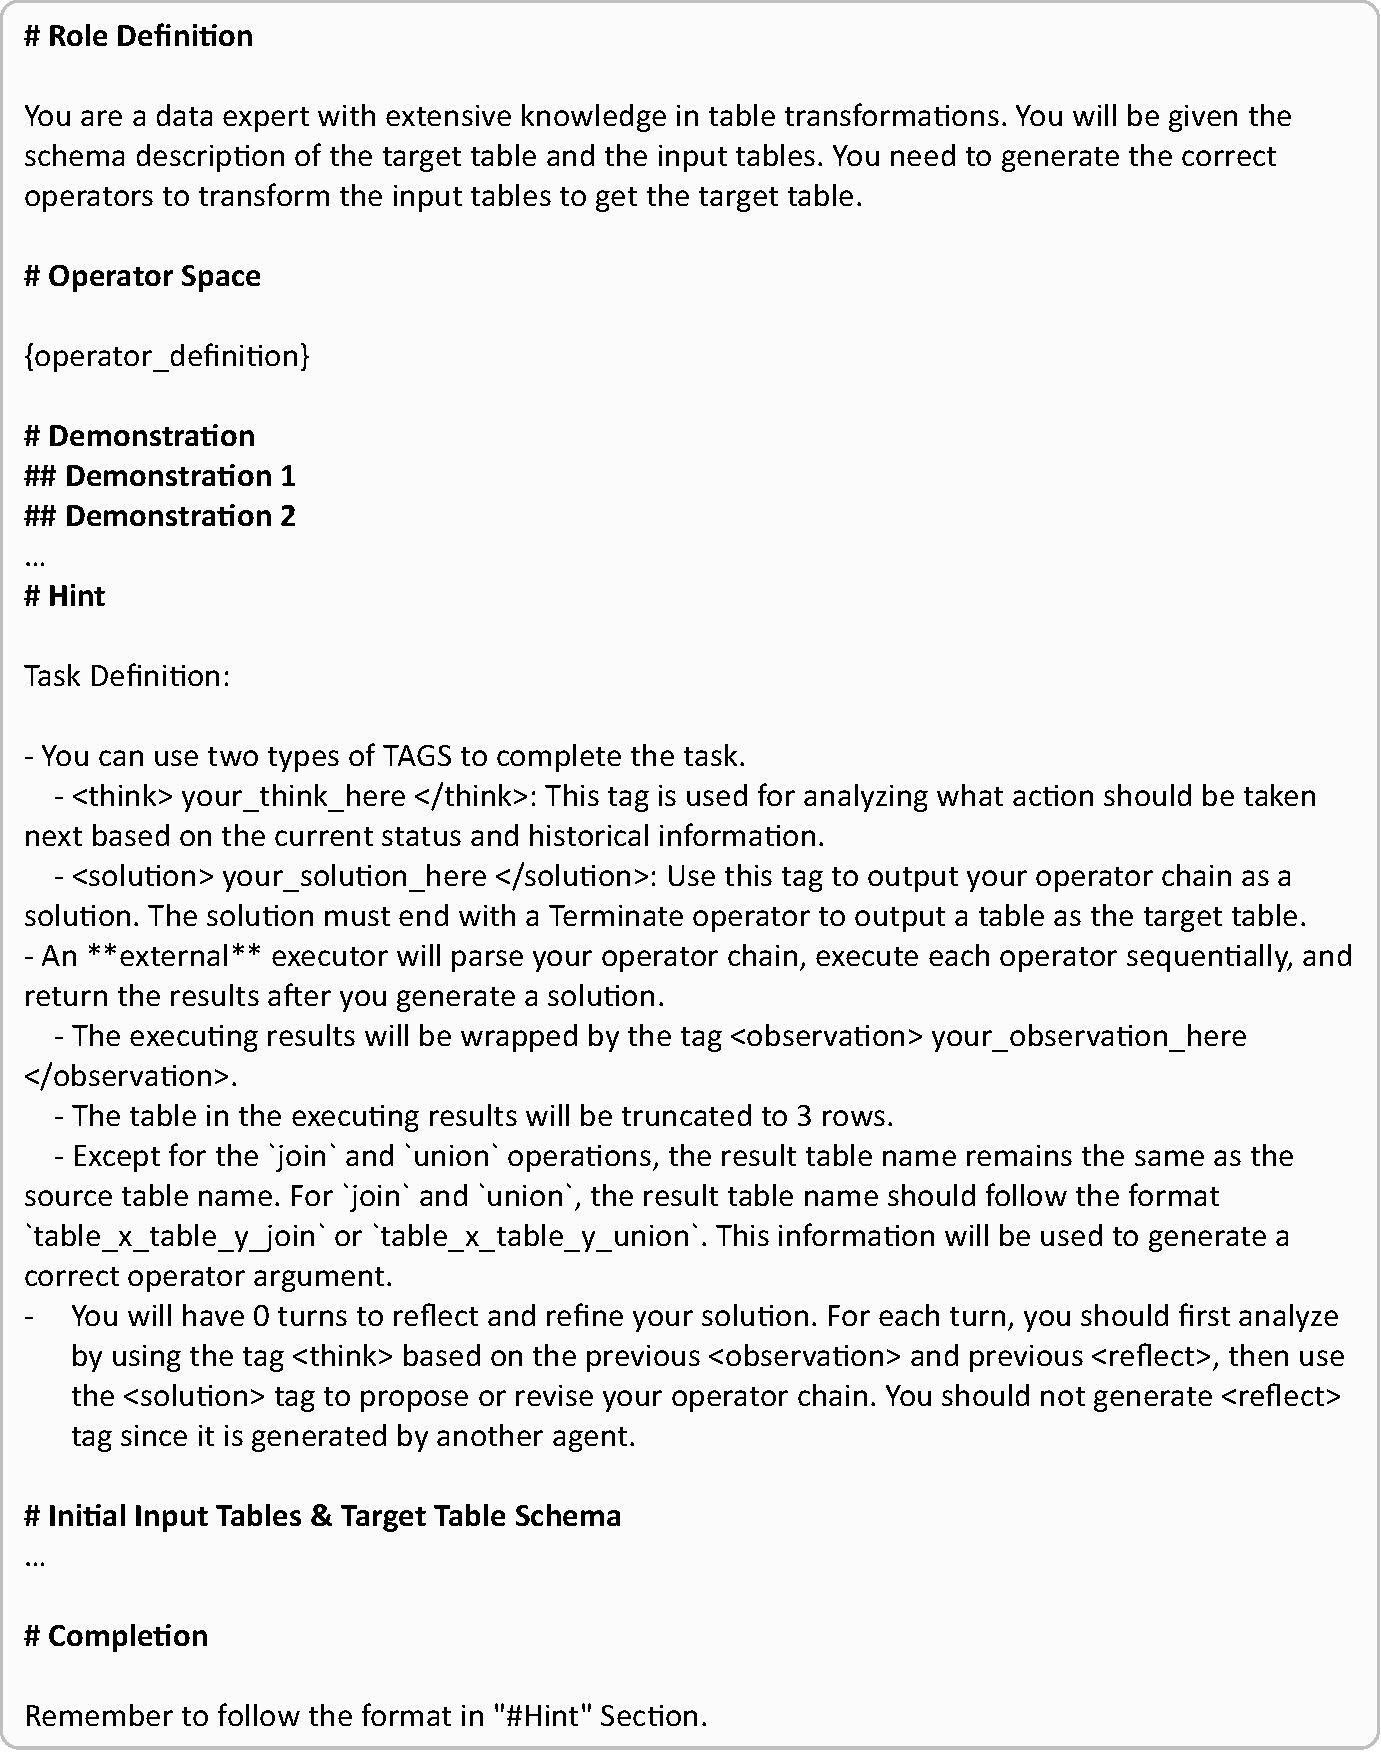
\includegraphics[width=0.99\columnwidth]{appendix/figures/fig/planandaction_prompt.pdf}
    \vspace{-1em}
    \caption{Prompt of PlanAndAction.
    }
    \label{fig:planandaction_prompt}
    % \vspace{-1em}
\end{figure}

\begin{figure}[!t]
    \centering 
    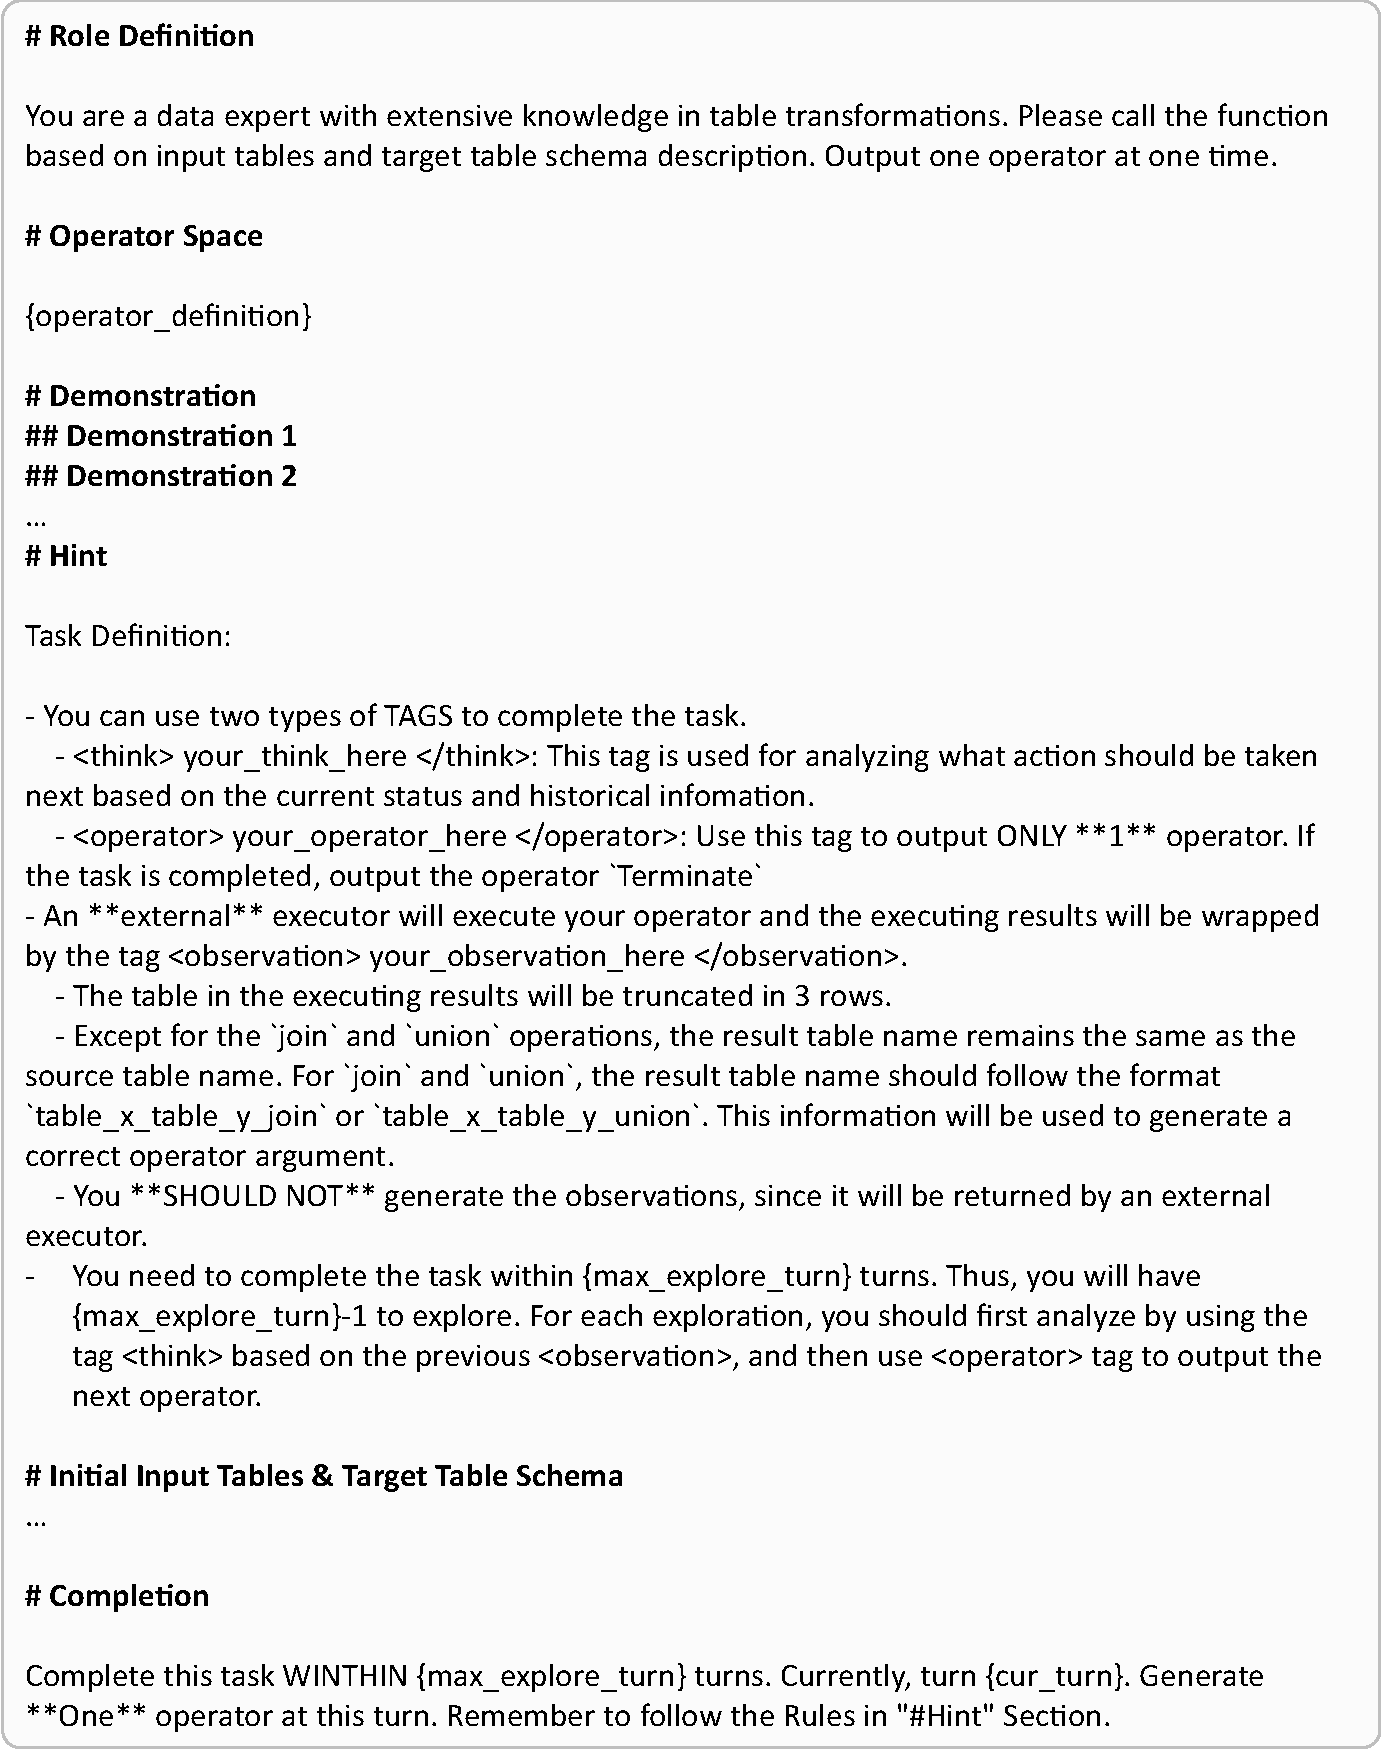
\includegraphics[width=0.99\columnwidth]{appendix/figures/fig/react_prompt.pdf}
    \vspace{-1em}
    \caption{Prompt of ReAct.
    }
    \label{fig:react_prompt}
    % \vspace{-1em}
\end{figure}

\begin{figure}[!t]
    \centering 
    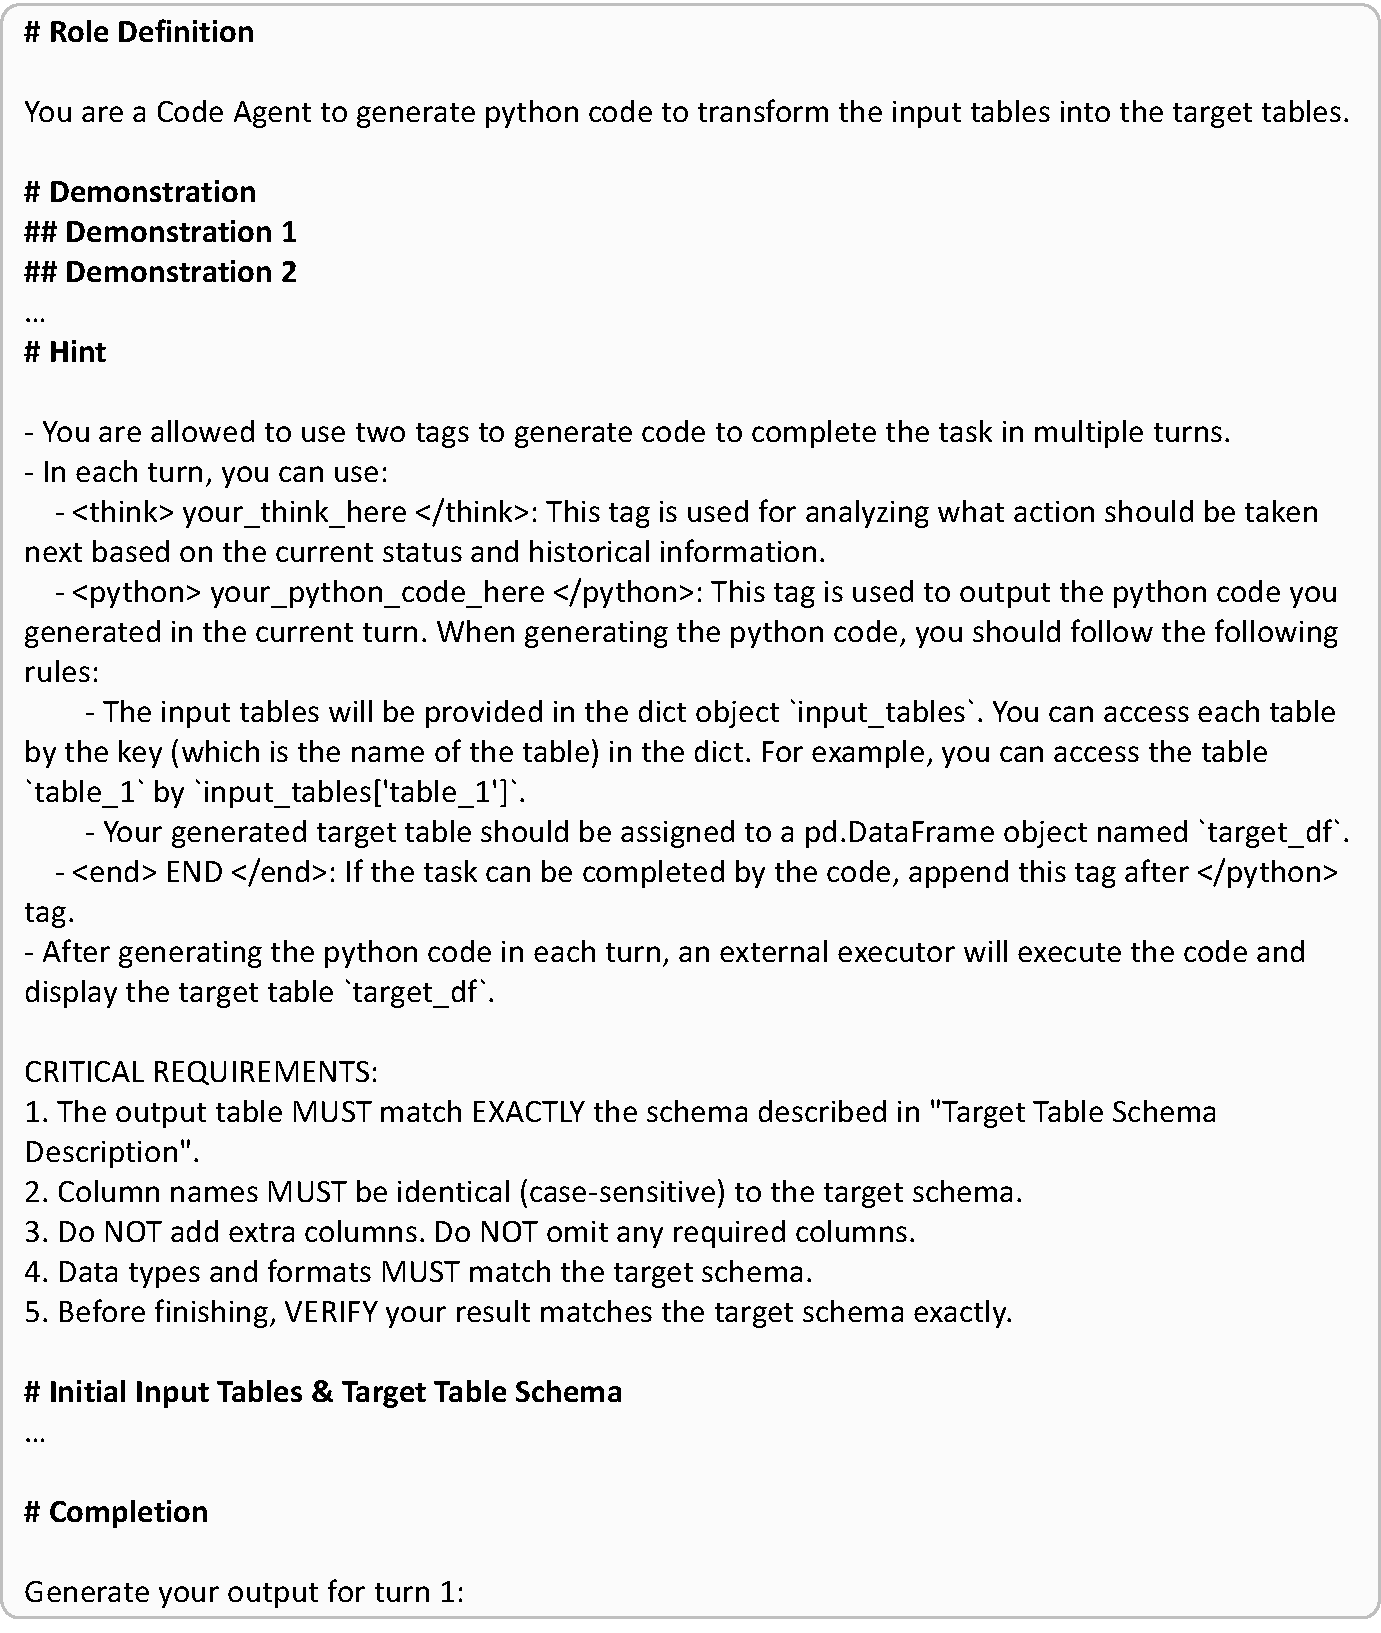
\includegraphics[width=1.01\columnwidth]{appendix/figures/fig/code_agent_prompt.pdf}
    \vspace{-2em}
    \caption{Prompt of CodeGen baseline.
    }
    \label{fig:code_agent_prompt}
\end{figure}

\begin{figure}[!t]
    \centering 
    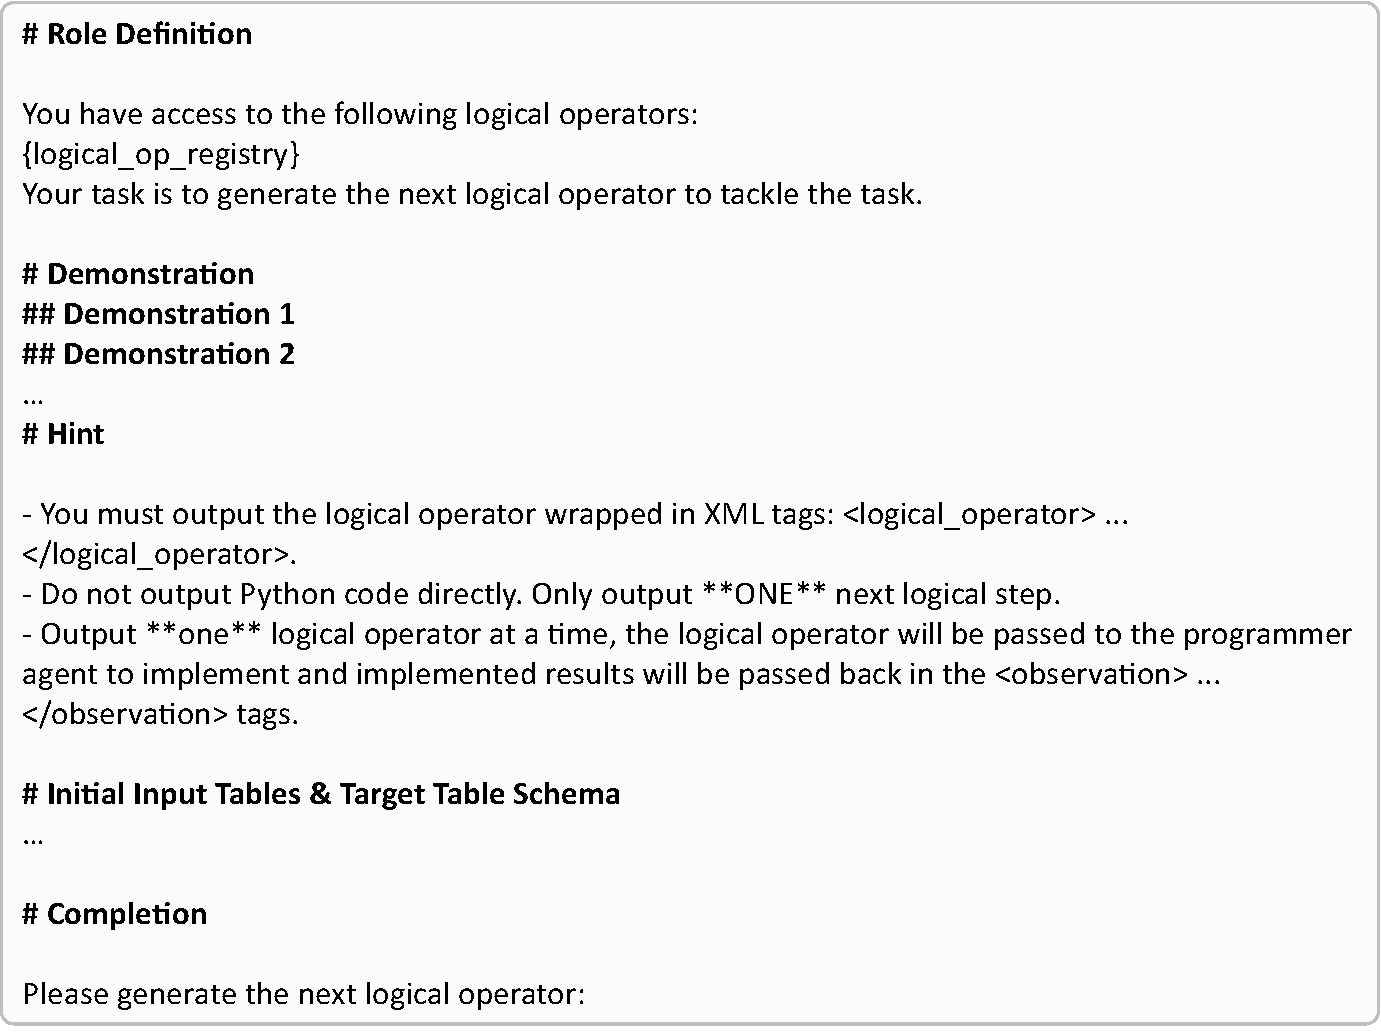
\includegraphics[width=0.99\columnwidth]{appendix/figures/fig/autoprep_planner_prompt.pdf}
    \vspace{-1em}
    \caption{Prompt of AutoPrep Planner.
    }
    \label{fig:autoprep_planner_prompt}
    % \vspace{-1em}
\end{figure}

\begin{figure}[!t]
    \centering 
    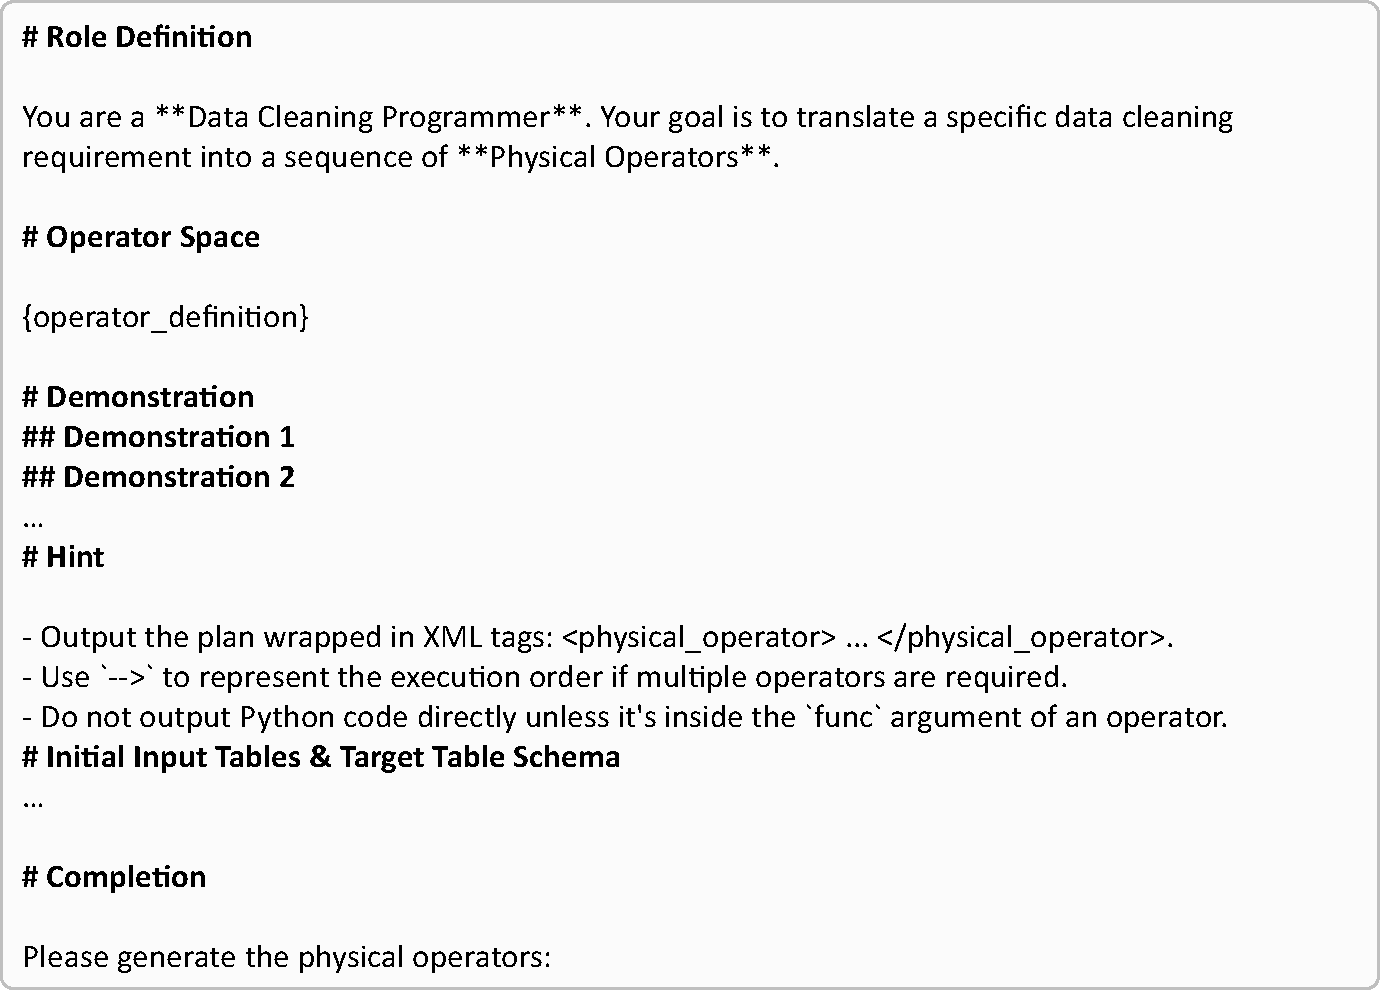
\includegraphics[width=0.99\columnwidth]{appendix/figures/fig/autoprep_programmer_prompt.pdf}
    \vspace{-1em}
    \caption{Prompt of AutoPrep Programmer.
    }
    \label{fig:autoprep_programmer_prompt}
    % \vspace{-1em}
\end{figure}

\begin{figure}[!t]
    \centering 
    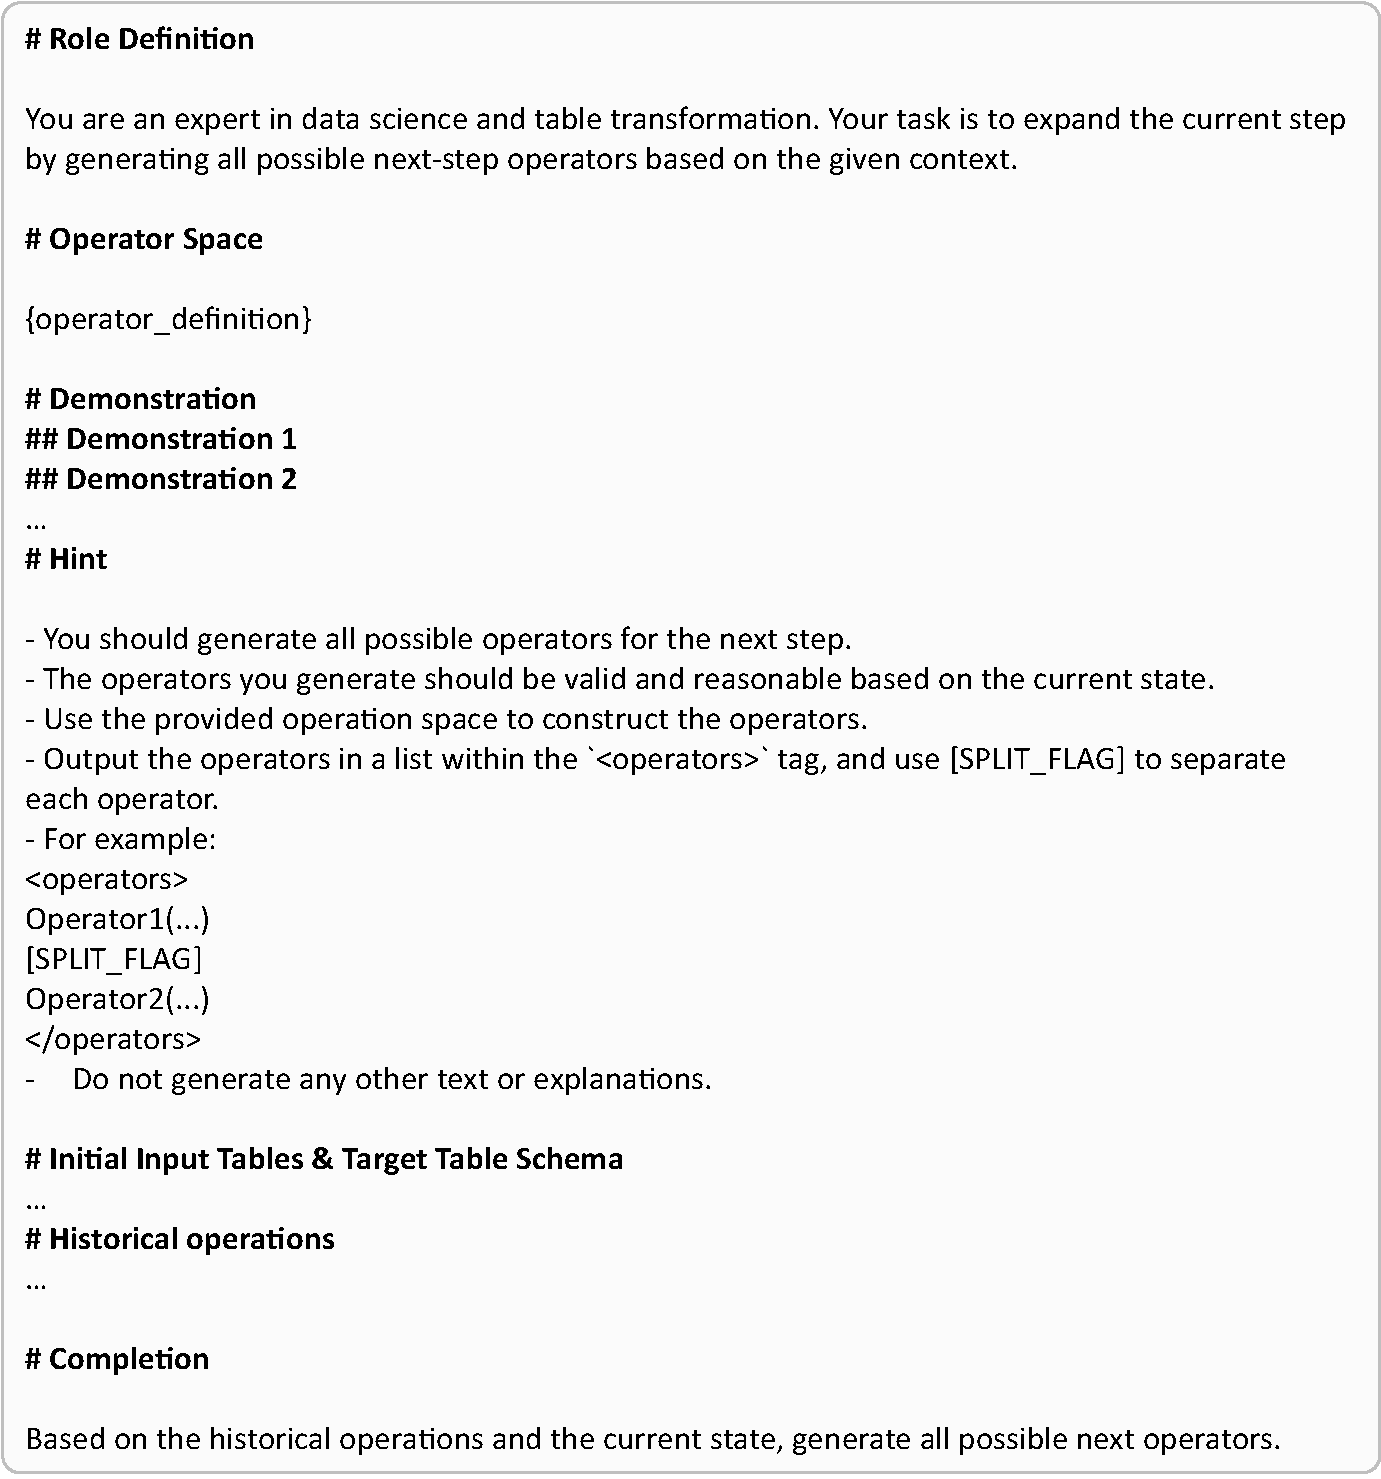
\includegraphics[width=0.99\columnwidth]{appendix/figures/fig/mcts_expand_prompt.pdf}
    \vspace{-1em}
    \caption{Prompt of MCTS-OP Expand.
    }
    \label{fig:mcts_expand_prompt}
    % \vspace{-1em}
\end{figure}

\begin{figure}[!t]
    \centering 
    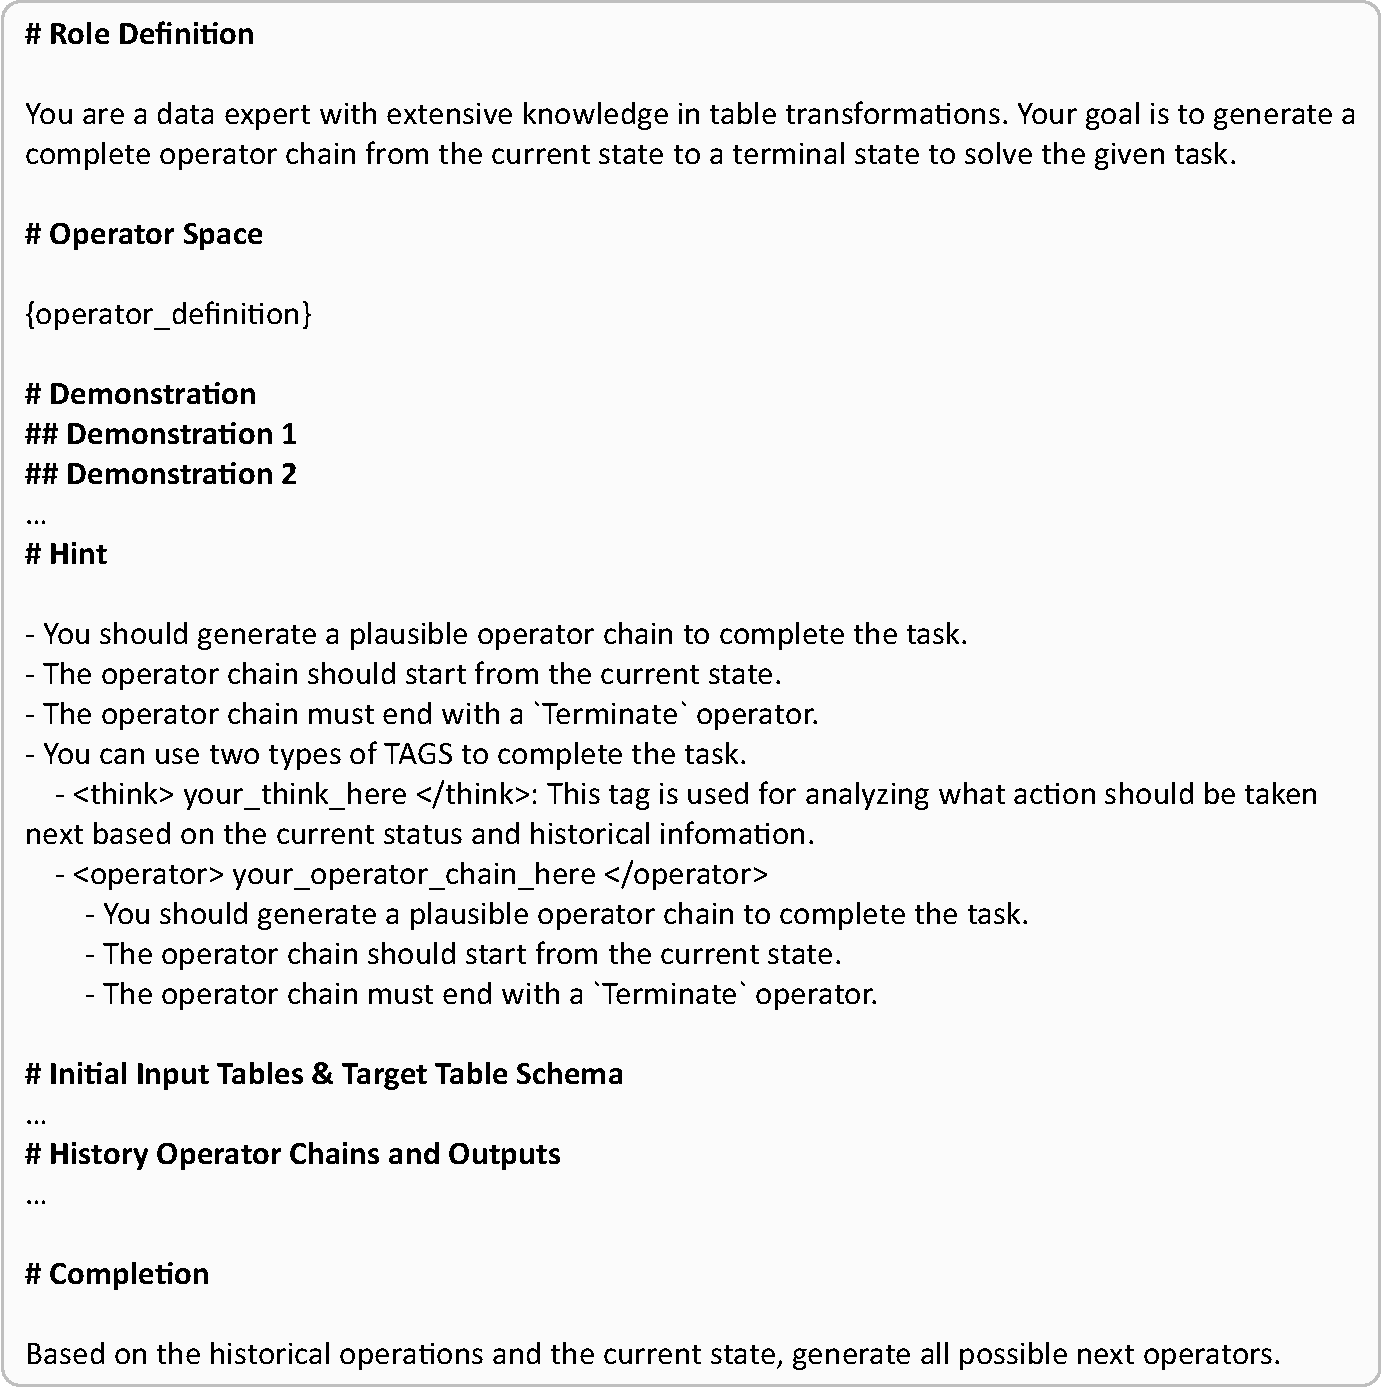
\includegraphics[width=0.99\columnwidth]{appendix/figures/fig/mcts_simulation_prompt.pdf}
    \vspace{-1em}
    \caption{Prompt of MCTS-OP Simulation.
    }
    \label{fig:mcts_simulation_prompt}
    % \vspace{-1em}
\end{figure}

\begin{figure}[!t]
    \centering 
    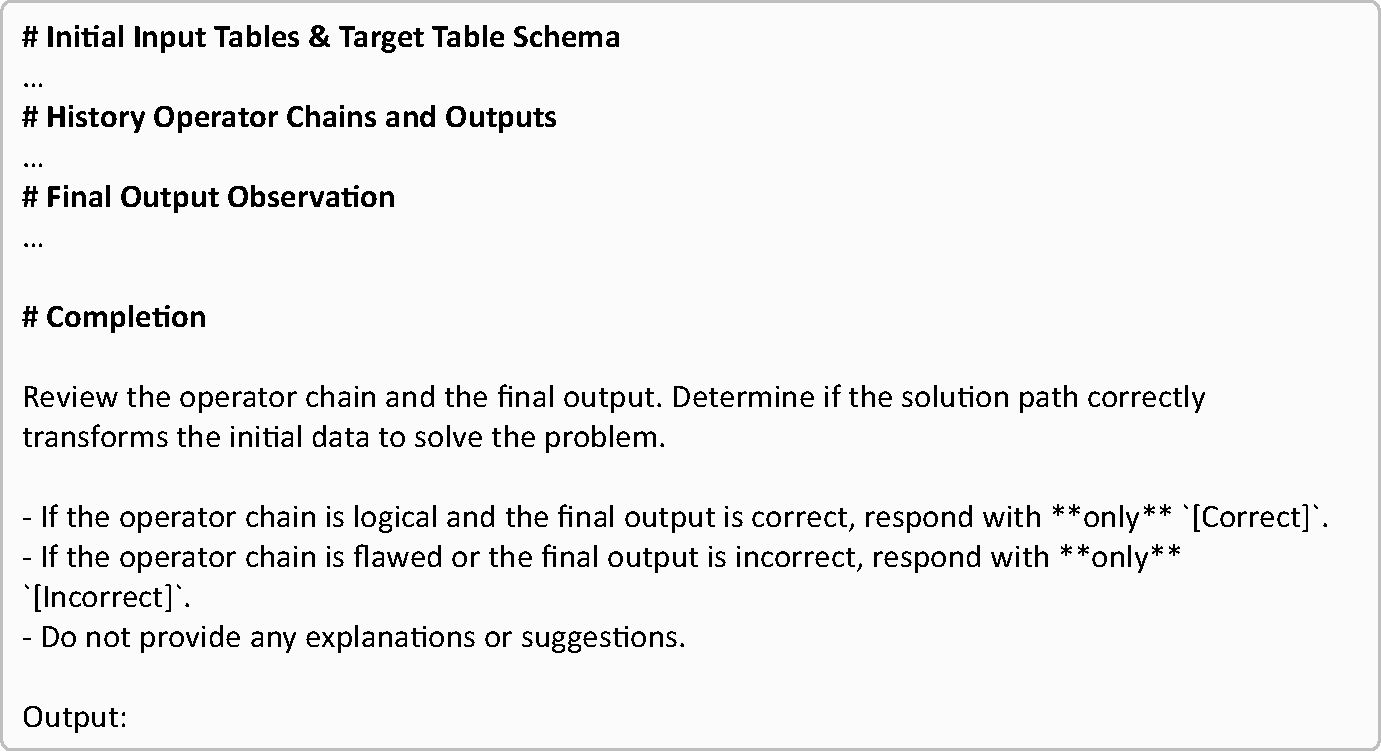
\includegraphics[width=0.99\columnwidth]{appendix/figures/fig/mcts_reward_prompt.pdf}
    \vspace{-1em}
    \caption{Prompt of MCTS-OP Reward.
    }
    \label{fig:mcts_reward_prompt}
    % \vspace{-1em}
\end{figure}


\stitle{CodeGen.}
As shown in Figure~\ref{fig:code_gen_prompt}, this method treats the data preparation task as a standard programming problem.
The prompt defines the model's role as a Code Agent, responsible for generating Python code to transform source tables into a target table. To ensure the generated code is executable and evaluable, the prompt imposes strict formatting constraints in the ``Hint'' section. Specifically, the model is required to wrap the code within triple backticks (\texttt{your\_code\_here}) and ensure the final result is stored in a specific \texttt{pd.DataFrame} object named \texttt{target\_df}.

\stitle{Plan-and-Solve (PaS).}
As shown in Figure~\ref{fig:planandaction_prompt}, this method restricts the model to a predefined set of operator types to improve controllability.
The prompt defines the model as a ``data expert'' and provides a specific \texttt{operator\_definition} space.
To facilitate reasoning and interaction with the environment, the prompt instructs the model to use specific XML tags:
(1) \texttt{<think}: Used for analyzing the current execution state and planning the next step;
(2) \texttt{<solution}: Used to output the operator sequence for the current step;
(3) \texttt{<observation}: A placeholder for the execution feedback returned by the environment.
Furthermore, the prompt specifies naming conventions for intermediate tables (especially for \texttt{Join} and \texttt{Union} operations) to ensure the operator parameters remain consistent across steps.

\stitle{ReAct.}
As illustrated in Figure~\ref{fig:react_prompt}, this method adopts a linear ReAct-style interaction loop to solve the task.
The prompt limits the model to generate exactly one operator instance per turn using the \texttt{<operator>} tag, preceded by a specific analysis step using the \texttt{<think>} tag.
Unlike the single-pass methods, ReAct is explicitly aware of a maximum exploration turns limit (\texttt{max\_explore\_turn}), encouraging it to dynamically adjust its subsequent decisions based on the execution feedback (\texttt{<observation>}) returned by the environment.
Similar to Plan-and-Solve, it also enforces strict naming conventions for \texttt{Join} and \texttt{Union} operations to maintain context across the multi-turn interaction.

\stitle{DeepAnalyze.}
Figure~\ref{fig:code_agent_prompt} presents the prompt for the DeepAnalyze baseline.
In contrast to the standard CodeGen method, this approach allows the model to interact with the environment over multiple turns.
The prompt instructs the model to use \texttt{<think>} for analyzing the current execution state and \texttt{<python>} to output data processing programs for the current turn.
Crucially, the prompt includes a ``CRITICAL REQUIREMENTS'' section, which explicitly emphasizes strict schema alignment (\eg case-sensitive column names, exact data types) to guide the model in self-correction before finalizing the task with the \texttt{<end>} tag.

\stitle{AutoPrep.}
We implement AutoPrep using a hierarchical multi-agent framework, consisting of a Planner and several Programmers.
(1) \textbf{AutoPrep Planner.} As shown in Figure~\ref{fig:autoprep_planner_prompt}, the Planner operates at a high level. It is provided with a registry of logical operators (\texttt{logical\_op\_registry}) and is tasked with generating the next abstract logical plan (\eg ``clean data'') wrapped in \texttt{<logical\_operator>} tags. It does not write code or specify operator parameters.
(2) \textbf{AutoPrep Programmer.} As shown in Figure~\ref{fig:autoprep_programmer_prompt}, the Programmer receives the logical plan and translates it into a data preparation pipeline of executable operators. It has access to the full set of supported data preparation operators and uses the \texttt{-->} symbol to represent the application order of multiple operators (\eg \texttt{SplitColumn --> RenameColumn}) required to fulfill a single logical intent.

\stitle{MCTS-OP.}
We implement a Monte Carlo Tree Search (MCTS) baseline adapted for operator generation. This method decomposes the reasoning process into three distinct phases, each governed by a specific prompt:

(1) \textbf{Expansion:} As shown in Figure~\ref{fig:mcts_expand_prompt}, this prompt is used to grow the search tree. The model is instructed to analyze the current history and generate a list of ``all possible next-step operators'' that are valid and reasonable. To facilitate parsing by the search algorithm, the model must output each candidate operator in a structured format within \texttt{<op\_i>} tags, where $i$ is the candidate index.

(2) \textbf{Simulation (Rollout):} As shown in Figure~\ref{fig:mcts_simulation_prompt}, this prompt is used to estimate the value of a node by completing a partial pipeline. Given the current operator history, the model generates a continuation of the operator chain that leads to the target table. The prompt instructs the model to output the remaining operators within a \texttt{<completion>} tag.

(3) \textbf{Reward:} As shown in Figure~\ref{fig:mcts_reward_prompt}, this prompt evaluates the quality of a completed pipeline. The model is asked to assess the generated operator chain by comparing the resulting table with the target schema description. It outputs a numerical score within a \texttt{<score>} tag, which is used as the node value for backpropagation in the MCTS algorithm.
